\subsubsection{Module MD-05: Quản lý Bán hàng Tại chỗ (POS - Eat-in)}
Module Quản lý Bán hàng Tại chỗ (MD-05), thường được biết đến với tên gọi Point of Sale (POS) cho dịch vụ ăn tại nhà hàng (Eat-in), là giao diện và hệ thống nghiệp vụ cốt lõi mà nhân viên phục vụ và thu ngân sử dụng để quản lý toàn bộ quy trình phục vụ khách hàng tại bàn. Từ việc mở ca làm việc, chọn bàn, nhận đơn hàng, gửi yêu cầu xuống bếp, xử lý các thay đổi, cho đến việc thanh toán và đóng đơn, module này đóng vai trò trung tâm trong hoạt động hàng ngày của nhà hàng.



\begin{figure}[H]
    \centering
    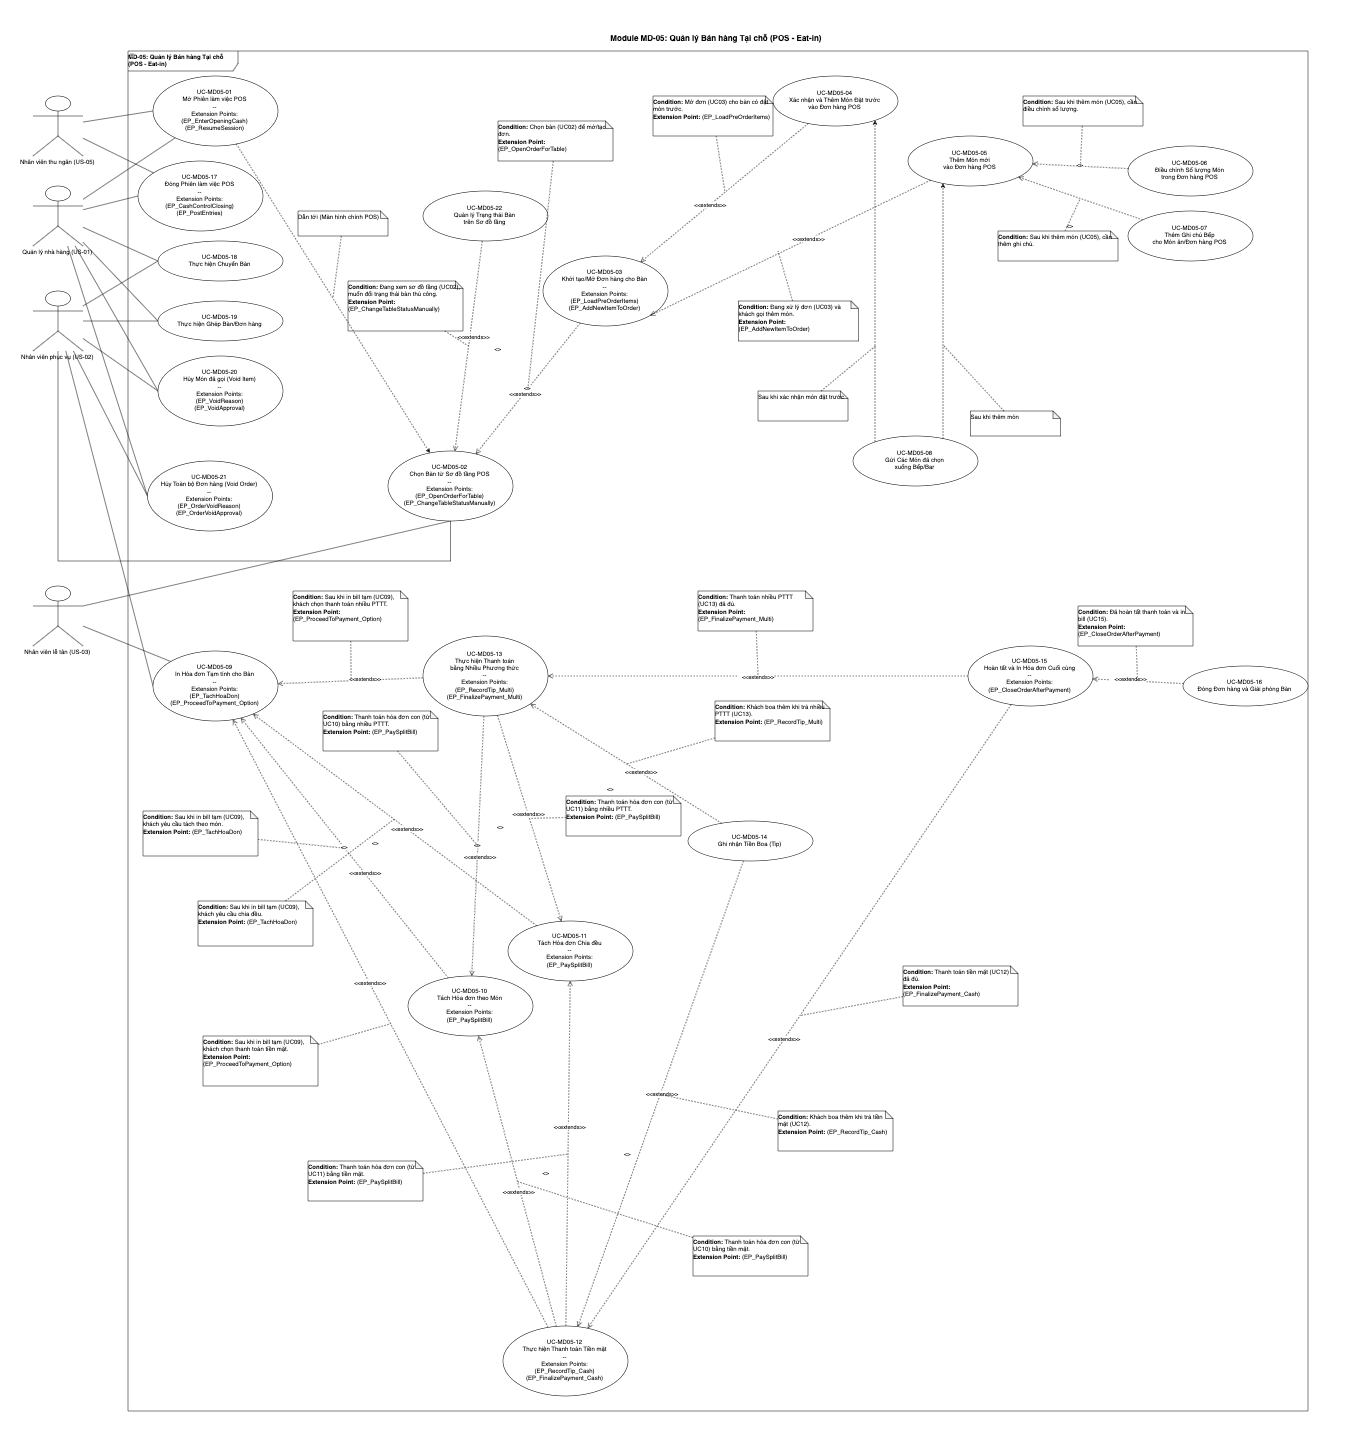
\includegraphics[width=15cm]{Sections/tong_quan/functional_spec/img/uc5.png}
    \vspace{0.5cm}
    \caption{Use case diagram cho Module MD-05}
    \label{fig:my_label}
\end{figure}

\begin{longtable}{|m{2cm}|m{2.5cm}|m{2cm}|m{4.5cm}|m{4cm}|}
\caption{Danh sách Yêu cầu Chức năng cho Module MD-05: Quản lý Bán hàng Tại chỗ (POS - Eat-in)} \label{tab:fr_md05_revised_v3_no_card} \\
\hline
\textbf{Mã Module} & \textbf{Mã Yêu cầu CN} & \textbf{Mã Người dùng} & \textbf{Tên Chức năng} & \textbf{Mô tả Ngắn} \\
\hline
\endhead % Header cho các trang tiếp theo
\hline
\endfoot % Footer cho bảng
\hline
\endlastfoot % Footer cho trang cuối cùng

MD-05 & FR-MD05-01 & US-05/US-01 & Mở Phiên làm việc POS & Cho phép Thu ngân/Quản lý bắt đầu phiên POS, nhập tiền mặt đầu ca. \\
\hline
MD-05 & FR-MD05-02 & US-02/US-03 & Chọn Bàn từ Sơ đồ tầng POS & Nhân viên chọn bàn trống hoặc bàn có khách/đặt trước từ sơ đồ tầng. \\
\hline
MD-05 & FR-MD05-03 & US-02 & Khởi tạo/Mở Đơn hàng cho Bàn & Hệ thống tạo đơn mới cho bàn trống hoặc mở đơn hiện có của bàn đang hoạt động/có đặt trước. \\
\hline
MD-05 & FR-MD05-04 & US-02 & Xác nhận và Thêm Món Đặt trước vào Đơn hàng POS & Nhân viên xem các món khách đã đặt trước (nếu có) và xác nhận thêm vào đơn hàng POS. \\
\hline
MD-05 & FR-MD05-05 & US-02 & Thêm Món mới vào Đơn hàng POS & Nhân viên chọn món từ menu POS để thêm vào đơn hàng hiện tại. \\
\hline
MD-05 & FR-MD05-06 & US-02 & Điều chỉnh Số lượng Món trong Đơn hàng POS & Nhân viên tăng/giảm số lượng một món đã có trong đơn hàng. \\
\hline
MD-05 & FR-MD05-07 & US-02 & Thêm Ghi chú Bếp cho Món ăn/Đơn hàng POS & Nhân viên thêm yêu cầu đặc biệt cho món hoặc cả đơn. \\
\hline
MD-05 & FR-MD05-08 & US-02 & Gửi Các Món đã chọn xuống Bếp/Bar & Nhân viên gửi các món mới thêm/món đặt trước đã xác nhận xuống bộ phận chuẩn bị. \\
\hline
MD-05 & FR-MD05-09 & US-02 & In Hóa đơn Tạm tính cho Bàn & Nhân viên in bill tạm tính (đã trừ cọc nếu có) cho khách kiểm tra. \\
\hline
MD-05 & FR-MD05-10 & US-02 & Tách Hóa đơn theo Món & Nhân viên chia hóa đơn của bàn theo từng món ăn cụ thể. \\
\hline
MD-05 & FR-MD05-11 & US-02 & Tách Hóa đơn Chia đều & Nhân viên chia đều tổng hóa đơn cho một số lượng người/phần nhất định. \\
\hline
MD-05 & FR-MD05-12 & US-02/US-05 & Thực hiện Thanh toán Tiền mặt & Nhân viên nhận tiền mặt, nhập số tiền nhận và hệ thống tính tiền thừa. \\
\hline
% FR-MD05-13 (Thanh toán thẻ) ĐÃ BỊ LOẠI BỎ
% Đánh số lại các FR tiếp theo
MD-05 & FR-MD05-13 & US-02/US-05 & Thực hiện Thanh toán bằng Nhiều Phương thức (Không bao gồm Thẻ) & Nhân viên nhận thanh toán cho một hóa đơn bằng cách kết hợp nhiều phương thức được hỗ trợ (ví dụ: Tiền mặt và Ví điện tử). \\
\hline
MD-05 & FR-MD05-14 & US-02/US-05 & Ghi nhận Tiền Boa (Tip) & Nhân viên nhập số tiền boa khách hàng trả thêm. \\
\hline
MD-05 & FR-MD05-15 & US-02/US-05 & Hoàn tất và In Hóa đơn Cuối cùng & Sau khi nhận đủ tiền, nhân viên xác nhận hoàn tất thanh toán và in hóa đơn/biên lai. \\
\hline
MD-05 & FR-MD05-16 & US-02 & Đóng Đơn hàng và Giải phóng Bàn & Nhân viên đóng đơn hàng đã thanh toán và cập nhật bàn thành trống. \\
\hline
MD-05 & FR-MD05-17 & US-05/US-01 & Đóng Phiên làm việc POS & Thu ngân/Quản lý kết thúc phiên, tổng kết, đối chiếu tiền mặt. \\
\hline
MD-05 & FR-MD05-18 & US-01/US-02 & Thực hiện Chuyển Bàn & Nhân viên chuyển toàn bộ đơn hàng từ bàn này sang bàn trống khác. \\
\hline
MD-05 & FR-MD05-19 & US-01/US-02 & Thực hiện Ghép Bàn/Đơn hàng & Nhân viên gộp nhiều đơn hàng từ các bàn khác nhau vào một bàn. \\
\hline
MD-05 & FR-MD05-20 & US-01/US-02 & Hủy Món đã gọi (Void Item) & Nhân viên hủy một món đã thêm vào đơn (có thể cần quyền). \\
\hline
MD-05 & FR-MD05-21 & US-01/US-02 & Hủy Toàn bộ Đơn hàng (Void Order) & Nhân viên hủy cả đơn hàng đang xử lý (có thể cần quyền). \\
\hline
MD-05 & FR-MD05-22 & US-02/ US-03 & Quản lý Trạng thái Bàn trên Sơ đồ tầng & Nhân viên có thể thay đổi thủ công trạng thái bàn (ví dụ: "Cần dọn", "Đang chờ") nếu cần. \\
\hline

\end{longtable}


\subsubsubsection{Mục tiêu và Phạm vi}
\label{sssec:md05_objectives_scope}
Mục tiêu chính của module MD-05 là:
\begin{itemize}
    \item \textbf{Tối ưu hóa quy trình phục vụ tại bàn:} Cung cấp một giao diện nhanh chóng, trực quan và dễ sử dụng cho nhân viên để nhận đơn, gửi bếp, và quản lý các yêu cầu của khách.
    \item \textbf{Quản lý bàn hiệu quả:} Hiển thị sơ đồ tầng trực quan với trạng thái bàn cập nhật theo thời gian thực, hỗ trợ việc xếp khách và theo dõi tình trạng phục vụ.
    \item \textbf{Đảm bảo tính chính xác của đơn hàng:} Giảm thiểu sai sót trong việc ghi nhận món ăn, số lượng, biến thể, và các yêu cầu đặc biệt của khách.
    \item \textbf{Tích hợp liền mạch với bếp/bar:} Gửi thông tin đơn hàng một cách chính xác và kịp thời đến các bộ phận chuẩn bị thông qua máy in hoặc Màn hình Hiển thị Bếp (KDS).
    \item \textbf{Linh hoạt trong thanh toán:} Hỗ trợ nhiều phương thức thanh toán, khả năng tách hóa đơn, và ghi nhận tiền boa.
    \item \textbf{Kiểm soát và báo cáo tài chính:} Ghi nhận tất cả các giao dịch, hỗ trợ đối chiếu tiền mặt cuối ca và cung cấp dữ liệu cho việc tạo các bút toán kế toán.
    \item \textbf{Nâng cao trải nghiệm khách hàng:} Thông qua việc phục vụ nhanh chóng, chính xác và khả năng đáp ứng linh hoạt các yêu cầu của khách.
\end{itemize}
Phạm vi của module bao gồm toàn bộ các hoạt động từ khi nhân viên mở phiên làm việc POS, quản lý đơn hàng cho từng bàn (tạo mới, thêm/sửa/hủy món, chuyển/ghép bàn), xử lý thanh toán, cho đến khi đóng phiên làm việc và tổng kết doanh thu.

\subsubsubsection{Đối tượng Sử dụng Chính}
\label{sssec:md05_primary_users}
Module này chủ yếu được sử dụng bởi các nhân viên tuyến đầu của nhà hàng:
\begin{itemize}
    \item \textbf{US-02 (Nhân viên phục vụ):} Là người dùng thường xuyên nhất, chịu trách nhiệm chính trong việc sử dụng sơ đồ tầng, nhận đơn hàng từ khách, thêm món, gửi yêu cầu bếp, và có thể cả việc nhận một phần thanh toán.
    \item \textbf{US-05 (Nhân viên thu ngân):} Chịu trách nhiệm mở và đóng phiên làm việc POS, xử lý các giao dịch thanh toán phức tạp, đối chiếu tiền mặt.
    \item \textbf{US-01 (Quản lý nhà hàng):} Có thể thực hiện tất cả các chức năng của nhân viên phục vụ và thu ngân, đồng thời có quyền thực hiện các hành động quản lý như hủy món/đơn hàng, chuyển/ghép bàn, và xem báo cáo phiên.
    \item \textbf{US-03 (Nhân viên lễ tân):} Có thể sử dụng sơ đồ tầng để xếp khách và mở đơn hàng ban đầu cho bàn.
\end{itemize}

\subsubsubsection{Các Chức năng Chính}
\label{sssec:md05_key_functionalities}
Module MD-05 cung cấp một bộ các chức năng toàn diện cho việc bán hàng tại chỗ, được mô tả chi tiết qua các Use Case sau:

\begin{itemize}
    \item \textbf{Quản lý Phiên làm việc POS (UC-MD05-01, UC-MD05-17):}
    \begin{itemize}
        \item Mở một phiên làm việc mới, tùy chọn nhập số dư tiền mặt đầu ca (UC-MD05-01).
        \item Đóng phiên làm việc cuối ca, tổng kết giao dịch, đối chiếu tiền mặt và ghi nhận bút toán (UC-MD05-17).
    \end{itemize}

    \item \textbf{Quản lý Bàn và Đơn hàng (UC-MD05-02, UC-MD05-03, UC-MD05-18, UC-MD05-19, UC-MD05-22):}
    \begin{itemize}
        \item Hiển thị và cho phép chọn bàn từ sơ đồ tầng trực quan với trạng thái cập nhật (UC-MD05-02).
        \item Khởi tạo một đơn hàng mới cho bàn trống/đặt trước hoặc mở lại đơn hàng đang hoạt động của bàn đã có khách (UC-MD05-03).
        \item Thực hiện chuyển toàn bộ đơn hàng từ bàn này sang bàn khác (UC-MD05-18).
        \item Thực hiện ghép các đơn hàng từ nhiều bàn vào một bàn đích duy nhất (UC-MD05-19).
        \item (Tùy chọn) Cho phép nhân viên thay đổi thủ công trạng thái của bàn trên sơ đồ tầng (ví dụ: "Cần dọn dẹp") (UC-MD05-22).
    \end{itemize}

    \item \textbf{Thao tác trên Đơn hàng (UC-MD05-04 đến UC-MD05-08, UC-MD05-20, UC-MD05-21):}
    \begin{itemize}
        \item Tự động tải và cho phép nhân viên xác nhận/thêm các món khách đã đặt trước online vào đơn hàng POS (UC-MD05-04).
        \item Thêm các món ăn/đồ uống mới vào đơn hàng từ menu trực quan, bao gồm cả việc chọn biến thể (UC-MD05-05).
        \item Điều chỉnh số lượng của một món đã có trong đơn hàng (UC-MD05-06).
        \item Thêm các ghi chú hoặc yêu cầu đặc biệt của khách cho từng món hoặc toàn bộ đơn hàng để gửi xuống bếp (UC-MD05-07).
        \item Gửi thông tin các món đã chọn (mới hoặc đặt trước) xuống các máy in bếp/bar hoặc màn hình KDS tương ứng (UC-MD05-08).
        \item Hủy một món cụ thể đã gọi trong đơn hàng (Void Item), có thể yêu cầu lý do và quyền quản lý (UC-MD05-20).
        \item Hủy toàn bộ một đơn hàng đang hoạt động (Void Order), thường yêu cầu quyền quản lý và lý do (UC-MD05-21).
    \end{itemize}

    \item \textbf{Xử lý Thanh toán (UC-MD05-09 đến UC-MD05-16):}
    \begin{itemize}
        \item In hóa đơn tạm tính cho khách kiểm tra, bao gồm cả việc trừ tiền đặt cọc đã thanh toán (nếu có) (UC-MD05-09).
        \item Tách hóa đơn theo từng món ăn cụ thể để nhiều người có thể trả riêng (UC-MD05-10).
        \item Tách hóa đơn bằng cách chia đều tổng giá trị cho một số lượng người nhất định (UC-MD05-11).
        \item Thực hiện thanh toán bằng tiền mặt, tính toán tiền trả lại (UC-MD05-12).
        \item Thực hiện thanh toán bằng nhiều phương thức khác nhau (không bao gồm thẻ tích hợp terminal) cho cùng một hóa đơn (UC-MD05-13).
        \item Ghi nhận số tiền boa (tip) do khách hàng trả thêm (UC-MD05-14).
        \item Sau khi nhận đủ thanh toán, hoàn tất giao dịch và in hóa đơn/biên lai cuối cùng cho khách (UC-MD05-15).
        \item Đóng đơn hàng đã thanh toán và giải phóng bàn, cập nhật trạng thái bàn thành trống (UC-MD05-16).
    \end{itemize}
\end{itemize}

\subsubsubsection{Tóm tắt Luồng Hoạt động Tổng thể}
\label{sssec:md05_overall_workflow}
Luồng hoạt động chính trong module Bán hàng Tại chỗ (POS) thường diễn ra như sau:
\begin{enumerate}
    \item \textbf{Bắt đầu ca làm việc:} Nhân viên thu ngân/Quản lý Mở Phiên làm việc POS (UC-MD05-01), nhập số dư tiền mặt đầu ca nếu cần.
    \item \textbf{Chọn bàn và mở đơn hàng:}
        \begin{itemize}
            \item Nhân viên phục vụ Chọn Bàn từ Sơ đồ tầng POS (UC-MD05-02) dựa trên tình trạng bàn (trống, đặt trước).
            \item Hệ thống Khởi tạo/Mở Đơn hàng cho Bàn (UC-MD05-03).
        \end{itemize}
    \item \textbf{Nhận yêu cầu gọi món từ khách:}
        \begin{itemize}
            \item Nếu bàn có đặt món trước, nhân viên Xác nhận và Thêm Món Đặt trước vào Đơn hàng POS (UC-MD05-04).
            \item Nhân viên Thêm Món mới vào Đơn hàng POS (UC-MD05-05) theo yêu cầu của khách.
            \item Điều chỉnh Số lượng Món (UC-MD05-06) hoặc Thêm Ghi chú Bếp (UC-MD05-07) nếu cần.
            \item Sau mỗi lượt gọi món hoặc khi cần, nhân viên Gửi Các Món đã chọn xuống Bếp/Bar (UC-MD05-08).
        \end{itemize}
    \item \textbf{Quản lý đơn hàng trong quá trình phục vụ (nếu có):}
        \begin{itemize}
            \item Khách yêu cầu chuyển bàn: Nhân viên Thực hiện Chuyển Bàn (UC-MD05-18).
            \item Nhiều nhóm khách muốn ngồi chung: Nhân viên Thực hiện Ghép Bàn/Đơn hàng (UC-MD05-19).
            \item Khách đổi ý/nhân viên nhập sai: Nhân viên Hủy Món đã gọi (Void Item) (UC-MD05-20).
            \item Khách rời đi/lỗi nghiêm trọng: Nhân viên/Quản lý Hủy Toàn bộ Đơn hàng (Void Order) (UC-MD05-21).
            \item Cập nhật trạng thái bàn thủ công (ví dụ: "Cần dọn"): Nhân viên Quản lý Trạng thái Bàn trên Sơ đồ tầng (UC-MD05-22).
        \end{itemize}
    \item \textbf{Khách yêu cầu thanh toán:}
        \begin{itemize}
            \item Nhân viên In Hóa đơn Tạm tính cho Bàn (UC-MD05-09).
            \item Nếu khách yêu cầu trả riêng: Nhân viên Tách Hóa đơn theo Món (UC-MD05-10) hoặc Tách Hóa đơn Chia đều (UC-MD05-11).
            \item Nhân viên nhận thanh toán bằng các phương thức: Thực hiện Thanh toán Tiền mặt (UC-MD05-12), hoặc Thực hiện Thanh toán bằng Nhiều Phương thức (UC-MD05-13).
            \item Nếu khách boa: Nhân viên Ghi nhận Tiền Boa (Tip) (UC-MD05-14).
        \end{itemize}
    \item \textbf{Hoàn tất giao dịch:}
        \begin{itemize}
            \item Sau khi nhận đủ tiền, nhân viên Hoàn tất và In Hóa đơn Cuối cùng (UC-MD05-15).
            \item Cuối cùng, nhân viên Đóng Đơn hàng và Giải phóng Bàn (UC-MD05-16).
        \end{itemize}
    \item \textbf{Kết thúc ca làm việc:} Nhân viên thu ngân/Quản lý Đóng Phiên làm việc POS (UC-MD05-17), tổng kết và đối chiếu.
\end{enumerate}
Module MD-05 là trung tâm của các hoạt động dịch vụ tại nhà hàng, đảm bảo quy trình diễn ra mượt mà, chính xác và hiệu quả.
